\documentclass[11pt]{article}

\usepackage[a4paper,margin=1in]{geometry}
\usepackage[T1]{fontenc}
\usepackage[utf8]{inputenc}
\usepackage{amsmath}
\usepackage{array}
\usepackage{booktabs}
\usepackage{caption}
\usepackage{enumitem}
\usepackage{float}
\usepackage{graphicx}
\usepackage{hyperref}
\usepackage{microtype}
\usepackage{tabularx}
\usepackage{titlesec}
\usepackage{xcolor}
\usepackage{fancyhdr}

\hypersetup{
    colorlinks=true,
    linkcolor=blue!50!black,
    urlcolor=blue!50!black
}

\captionsetup{
    font=small,
    labelfont=bf
}
\captionsetup[table]{labelformat=empty,labelsep=none}

\setlist{nosep,leftmargin=1.6em}
\setlength{\parskip}{0.4em}
\setlength{\parindent}{0pt}
\setlength{\headheight}{14pt}
\renewcommand{\arraystretch}{1.15}
\raggedbottom

\titleformat{\section}
{\large\bfseries}
{\thesection}
{0.6em}
{}

\titleformat{\subsection}
{\normalsize\bfseries}
{\thesubsection}
{0.6em}
{}

\titlespacing*{\section}{0pt}{0.9em}{0.4em}
\titlespacing*{\subsection}{0pt}{0.7em}{0.3em}

\pagestyle{fancy}
\fancyhf{}
\lhead{}
\rhead{}
\renewcommand{\headrulewidth}{0pt}

\title{
    \vspace{-1.2em}
    \textbf{Improving Counting Sort via Data Locality}\\
    \large Cache-aware Hybrid Sorting with Modified Quicksort Preprocessing
}
\author{Group 13}
\date{}

\begin{document}

    \maketitle
    \thispagestyle{empty}

    \section{Introduction}

    This project implements and tests the algorithm from Paper 2. The paper tries to make counting
    sort faster by improving data locality. In theory, counting sort has the same $O(n + r)$ time
    bound for random and sorted input. In practice, though, random input can still run much slower.

    The paper explains this using memory access. Counting sort updates
    \texttt{count[value]} again and again. When the values are spread out, these updates jump
    around memory and cause more cache misses. When nearby values update nearby counters, the work
    stays in a smaller area of memory and becomes cheaper.

    We test that idea on our own machine using a Java implementation and compare the results with
    the paper's three benchmark groups.


    \section{The Hybrid Method}

    Instead of running one global counting-sort pass, Paper 2 uses a two-stage method:

    \begin{enumerate}
        \item \textbf{Preprocess with modified quicksort.} Partition using median-of-three pivots.
        \item \textbf{Early stop using threshold rule.} Stop recursion when
        \[
            (\max - \min) + \text{size} \leq C.
        \]
        \item \textbf{Partition-local counting sort.} Run counting sort separately in each accepted partition.
    \end{enumerate}

    The goal is simple: spend some time reorganizing the data first, then make the counting stage
    cheaper by working on smaller and more cache-friendly ranges.

    \subsection{How It Differs from the Baselines}

    Compared with classic counting sort, the hybrid uses several small local count arrays instead
    of one large global one. Compared with full quicksort, it stops early and switches to counting
    sort once a partition is small enough in both size and value range. This helps most when cache
    pressure is high. It helps less when the preprocessing cost is bigger than the gain.

    \subsection{Complexity}

    The preprocessing step still behaves like quicksort, so the average case is $O(n\log n)$.
    It also keeps the usual quicksort worst-case risk if the splits are very uneven. The main
    benefit here is practical speed from better memory locality, not a better asymptotic bound.

    \section{Implementation Details}

    The repository is split into three main Java files. The core hybrid sorter is in
    \texttt{src/Improved\_CountingSort.java}. The benchmark and baseline driver is in
    \texttt{test/Improved\_CountingSortTest.java}. The threshold sweep tool is in
    \texttt{src/Improved\_CountingSortThresholdSweep.java}.

    \subsection{Code Organization}

    This structure keeps the sorter focused on the algorithm itself. Tasks like input generation,
    warm-up runs, timing, and baseline comparisons are kept outside it. That made the code easier
    to read and made it less likely that benchmark code would affect the algorithm.

    \subsection{Paper-to-Code Mapping}

    \begin{table}[H]
        \centering
        \caption{Mapping from paper concepts to implementation units.}
        \label{tab:mapping}
        \small
        \begin{tabularx}{\textwidth}{>{\raggedright\arraybackslash}p{4.0cm} >{\raggedright\arraybackslash}X}
            \toprule
            Paper concept & Implementation mapping \\
            \midrule
            Hybrid entry point & \texttt{sort(arr)} and \texttt{sort(arr, threshold)} \\
            Preprocessing stage & \texttt{preprocess(...)} + \texttt{quicksortModified(...)} \\
            Median-of-three pivot & \texttt{partitionMedianOfThreeWithBounds(...)} \\
            Early-stop rule & condition \texttt{max - min + size <= threshold} \\
            Partition descriptors & \texttt{PartitionPlan} and \texttt{Partition(low, high, minValue, maxValue)} \\
            Local counting pass & \texttt{countingSortPartitions(...)} and \texttt{countingSortPartition(...)} \\
            \bottomrule
        \end{tabularx}
        \normalsize
    \end{table}

    \subsection{How the Code Works}

    The paper gives the main idea, but the Java code needs a clear step-by-step flow.
    \texttt{sort(arr, threshold)} first checks that the threshold is valid and returns early for
    very small inputs. It then calls \texttt{preprocess(...)} to run the modified quicksort stage
    and build a \texttt{PartitionPlan}. This plan lists the partitions that will later be sorted
    by local counting sort.

    Each \texttt{Partition} stores both index bounds (\texttt{low}, \texttt{high}) and value
    bounds (\texttt{minValue}, \texttt{maxValue}). We keep these value bounds during
    preprocessing because the counting stage needs them later. This avoids recomputing them after
    partitioning. Recursion stops when the paper's condition
    \[
        (\max - \min) + \text{size} \leq C
    \]
    is true for the current segment.

    If a segment does not satisfy that rule, \texttt{partitionMedianOfThreeWithBounds(...)} splits
    it and at the same time tracks the largest value on the left and the smallest value on the
    right. That avoids an extra scan after each split. Pivot positions are stored as one-element
    partitions so the final plan still covers the whole array in order.

    The second stage, \texttt{countingSortPartitions(...)}, goes through the partition plan and
    sorts each accepted region separately. Inside \texttt{countingSortPartition(...)}, values are
    shifted by subtracting \texttt{minValue}. This means the local count array only covers the
    local value range, not the full global range. That is what makes the method more
    cache-friendly than classic counting sort.

    \subsection{Design Decisions}

    \textbf{Configurable threshold.} We keep $C=1000$ as the default because that matches the
    paper. We also allow other values and include a sweep tool, because the best choice of $C$
    depends on the machine.

    \textbf{Explicit partition metadata.} \texttt{PartitionPlan} makes the preprocessing stage
    easier to inspect and debug. It also lets the benchmark harness time preprocessing and
    counting separately for Table 2 style comparisons.

    \textbf{Bound propagation during partitioning.} The helper
    \texttt{partitionMedianOfThreeWithBounds(...)} keeps track of tighter left and right value
    bounds while it partitions. This means we do not need to rescan subarrays to recover local
    minima and maxima.

    \textbf{Value normalization in local counting sort.} Each partition offsets values by
    \texttt{minValue}, so the bucket array only covers the local value range. This keeps the local
    counting pass smaller.

    \textbf{Baseline reproduction in one harness.} The benchmark driver contains classic counting
    sort, classic quicksort, and quicksort with insertion sort in the same file as the experiment
    loops. Using one harness with fixed seeds and the same timing structure makes the comparisons
    fairer.

    \textbf{Filling in missing paper details.} The paper does not fully specify every experimental
    detail, so we had to make some choices. For example, the quicksort+insertion baseline uses a
    cutoff of 32, and the threshold sweep tool was added to explore different values of $C$.

    \textbf{Input validation.} Invalid thresholds are rejected early instead of causing problems
    later in the pipeline.

    \section{Experiments}

    All reported results come from benchmark methods in
    \texttt{test/Improved\_CountingSortTest.java} and were recorded in
    \texttt{your\_benchmark\_output.txt}.

    \subsection{Protocol}

    For each case, we use 3 warm-up runs and 10 measured runs. We time them with
    \texttt{System.nanoTime()} and report the average in milliseconds. Arrays are generated with
    fixed seeds so the runs are repeatable.

    \subsection{Workloads}

    \textbf{Table 1 style (input-order sensitivity).} We compare classic counting sort on random
    and sorted data with $n=r$ over larger and larger input sizes.

    \textbf{Table 2 style ($r \gg n$ stress test).} We compare the hybrid and classic counting
    sort with $r=1{,}000{,}000$ and $n$ from 1000 to 50,000. We also run a Table 2.2 version with
    a larger range, $r=100{,}000{,}000$, to put more pressure on the cache.

    \textbf{Table 3 style (quicksort variants).} We compare classic quicksort,
    quicksort+insertion, and quicksort+counting for $n=r$ up to 25 million.

    \subsection{Machine Used}

    We ran the experiments on an Intel Core i7-14650HX (16 cores) with Windows 11 and
    Temurin JDK 17.0.18. The cache hierarchy is L1 1.4 MB, L2 24 MB, and L3 30 MB. Exact timings
    depend on the hardware and the JVM, so our main goal was to match the paper's overall trends.

    \section{Results}

    \subsection{Main Results}

    \begin{table}[H]
        \centering
        \caption{Representative results from the current repository run.}
        \label{tab:key-results}
        \small
        \begin{tabularx}{\textwidth}{>{\raggedright\arraybackslash}p{2.2cm} >{\raggedright\arraybackslash}p{3.8cm} >{\raggedright\arraybackslash}X}
            \toprule
            Benchmark & Case & Observation \\
            \midrule
            Table 1 & $n=r=25$M & Random: 659.512 ms; Sorted: 105.319 ms ($\sim$6.26$\times$ gap). \\
            Table 2.1 & $r=1{,}000{,}000$ & Hybrid wins at $n=1000$ (0.210 vs 0.652 ms), then classic leads from $n=2000$ onward. \\
            Table 2.2 & $r=100{,}000{,}000$ & Hybrid remains faster across tested $n$ (e.g., at $n=500{,}000$: 82.076 ms vs classic 89.531 ms). \\
            Table 3 & $n=r=10$M & quicksort: 749.368 ms; quick+insertion: 656.226 ms; quick+counting: 473.387 ms ($\sim$1.58$\times$ vs quicksort). \\
            \bottomrule
        \end{tabularx}
        \normalsize
    \end{table}

    \subsection{Graphs}

    \begin{figure}[H]
        \centering
        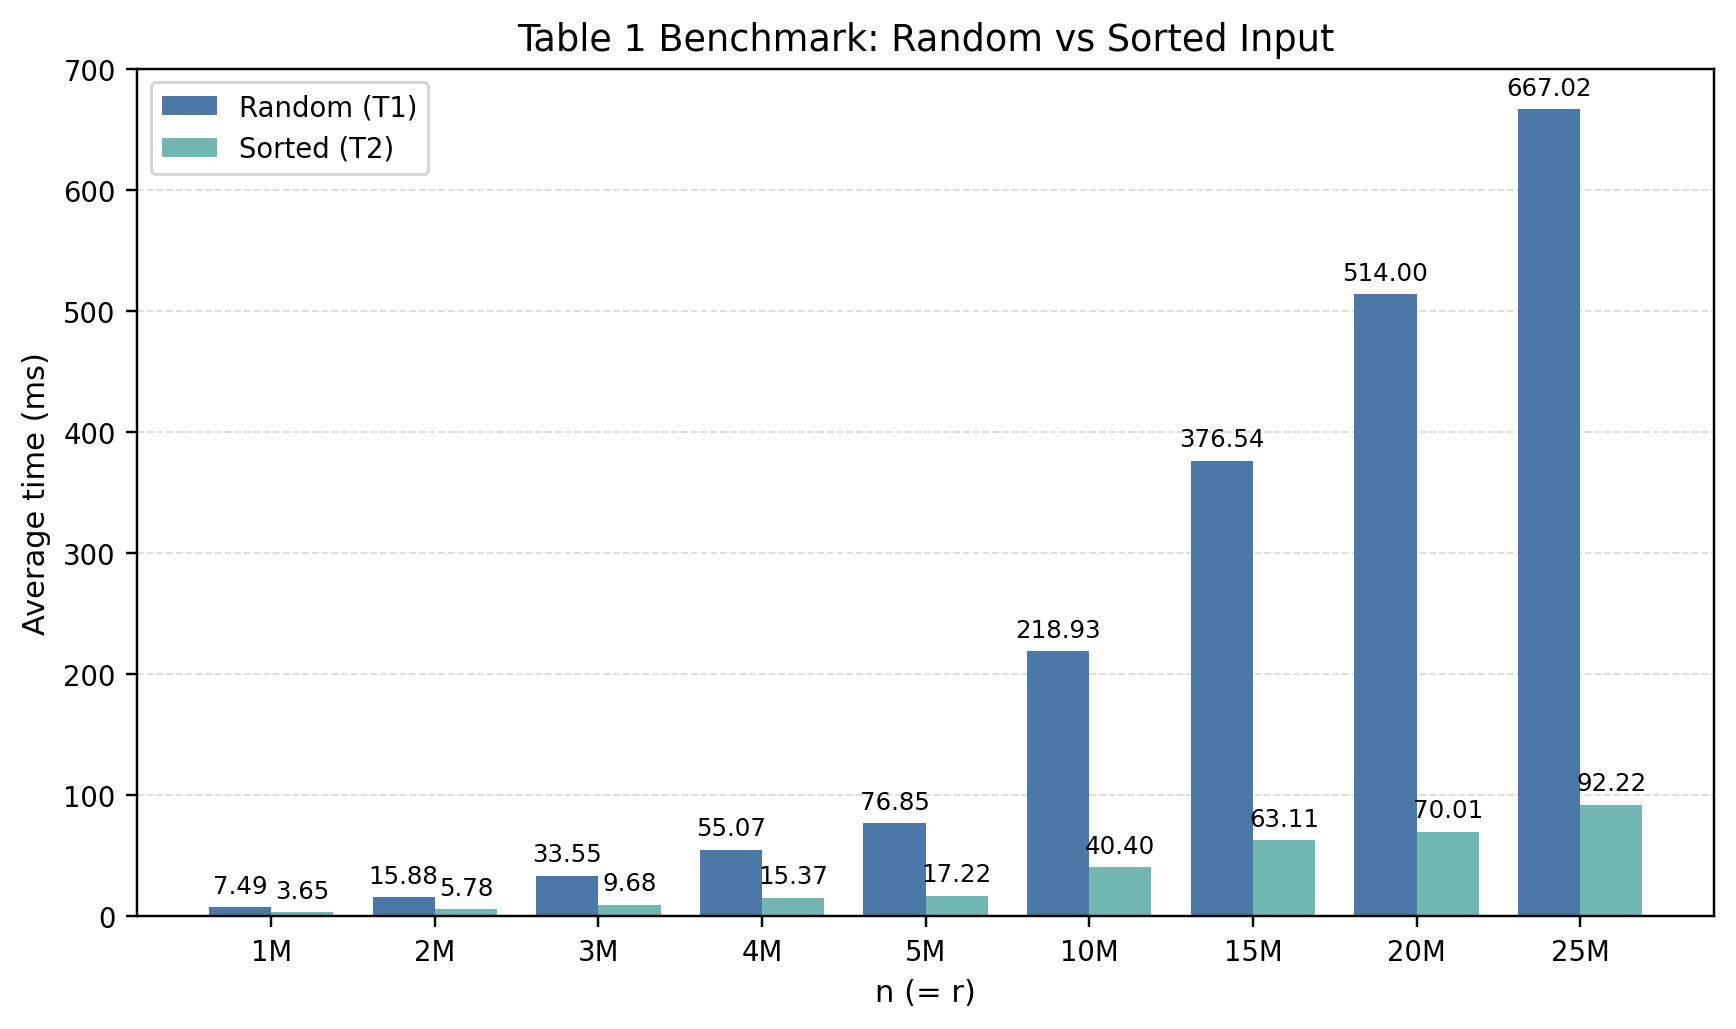
\includegraphics[width=0.78\textwidth]{graphs/table1_random_vs_sorted_ms.png}
        \caption{Table 1 trend: sorted input is much faster than random input.}
        \label{fig:table1trend}
    \end{figure}

    \begin{figure}[H]
        \centering
        \begin{minipage}[t]{0.49\textwidth}
            \centering
            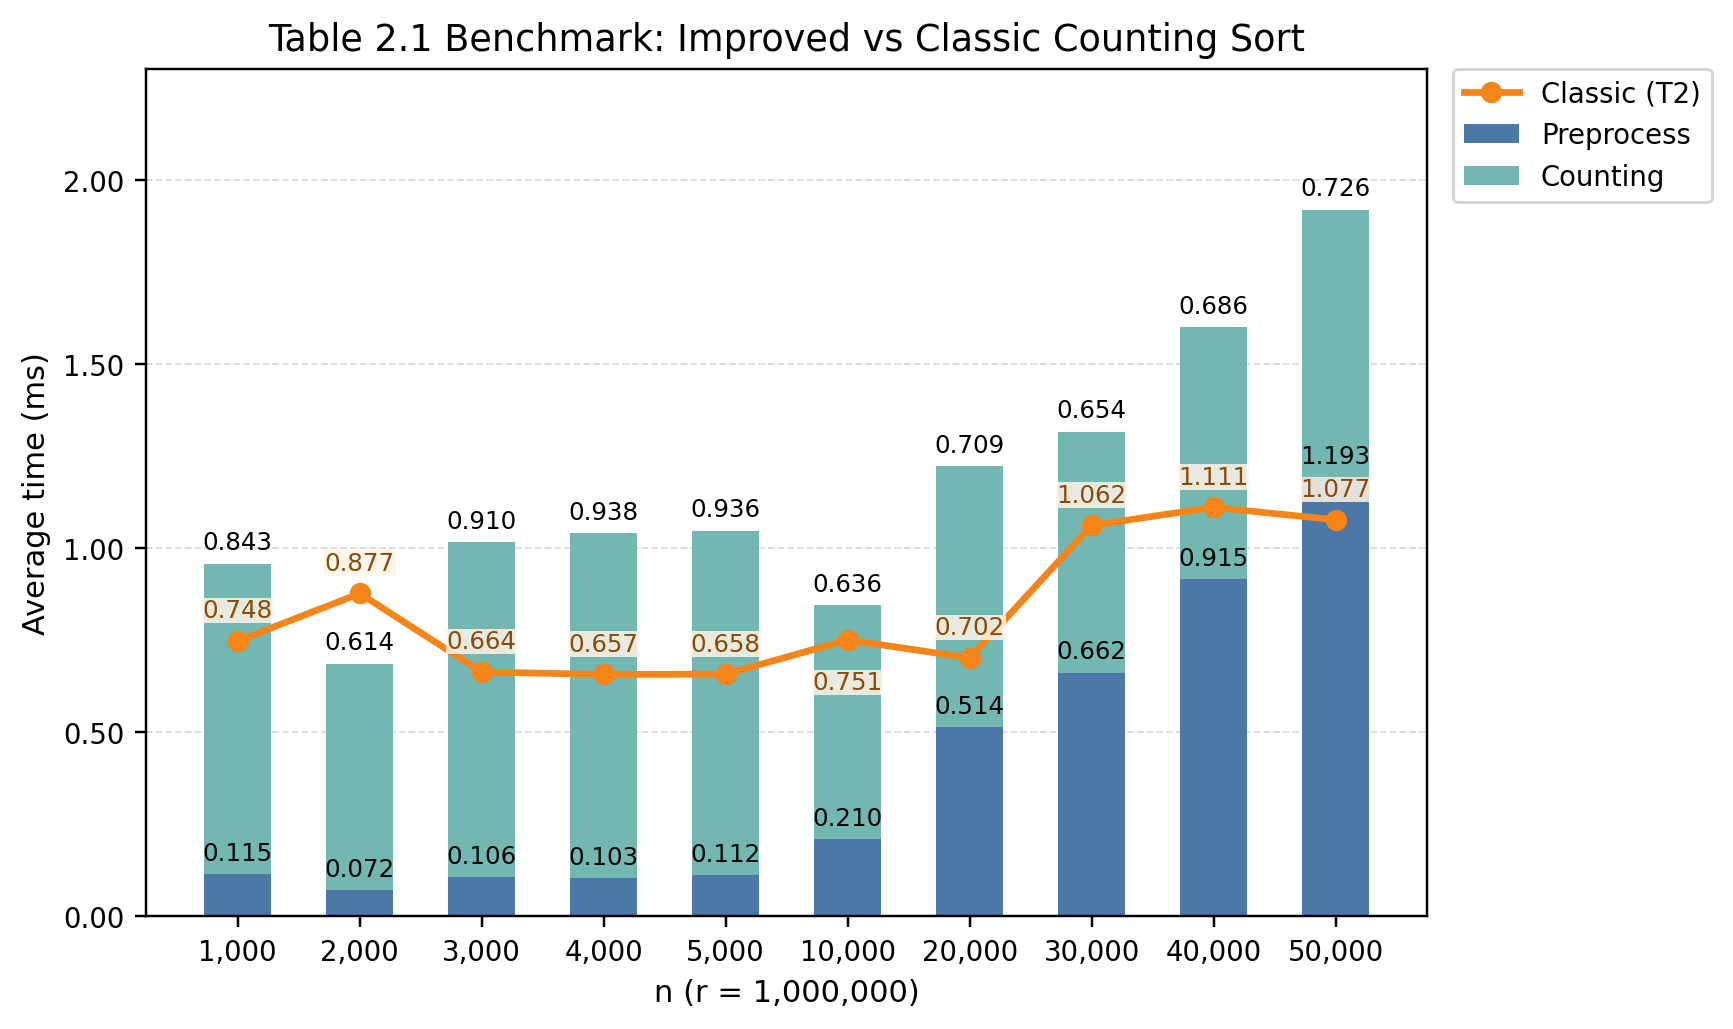
\includegraphics[width=\textwidth]{graphs/table2_1_preprocess_counting_vs_classic_ms.png}
            \caption*{(a) Table 2.1 ($r=1{,}000{,}000$): preprocessing cost is bigger than the
            gain for most of the small-$n$ cases.}
        \end{minipage}
        \hfill
        \begin{minipage}[t]{0.49\textwidth}
            \centering
            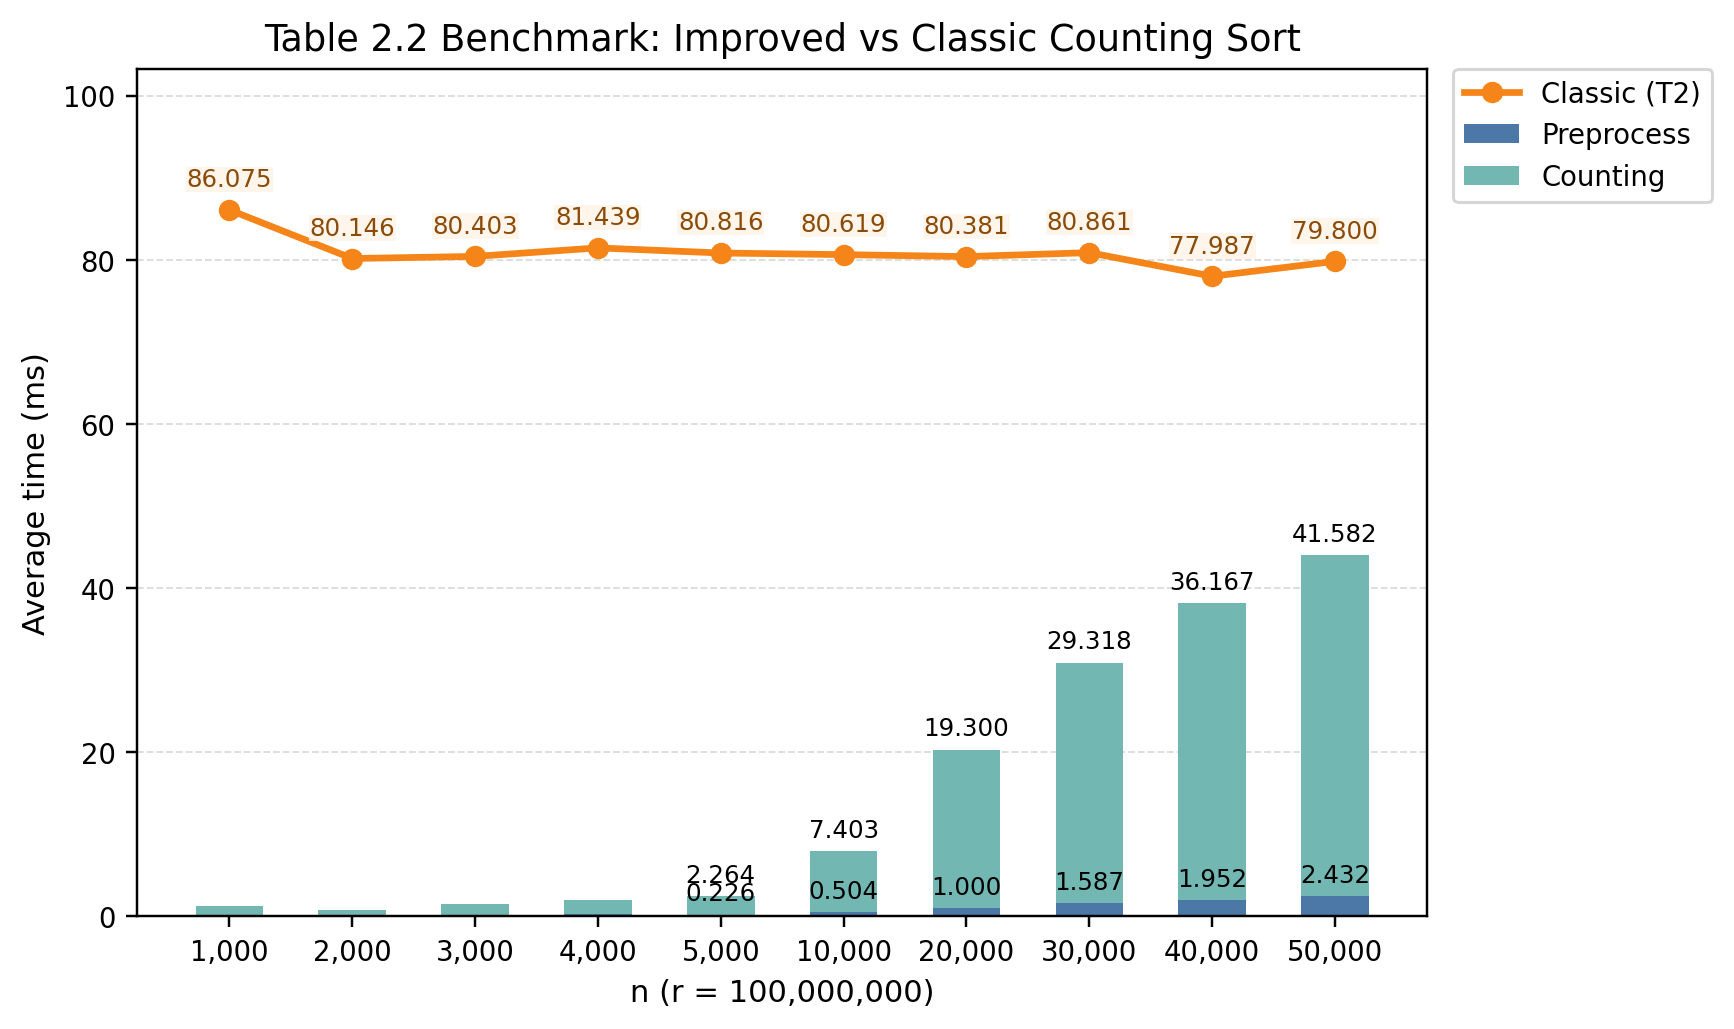
\includegraphics[width=\textwidth]{graphs/table2_2_preprocess_counting_vs_classic_ms.png}
            \caption*{(b) Table 2.2 ($r=100{,}000{,}000$): once classic counting sort becomes
            limited by cache, the hybrid pulls ahead.}
        \end{minipage}
        \caption{Table 2 trends shown side by side for easier comparison.}
        \label{fig:table2trends}
    \end{figure}

    \begin{figure}[H]
        \centering
        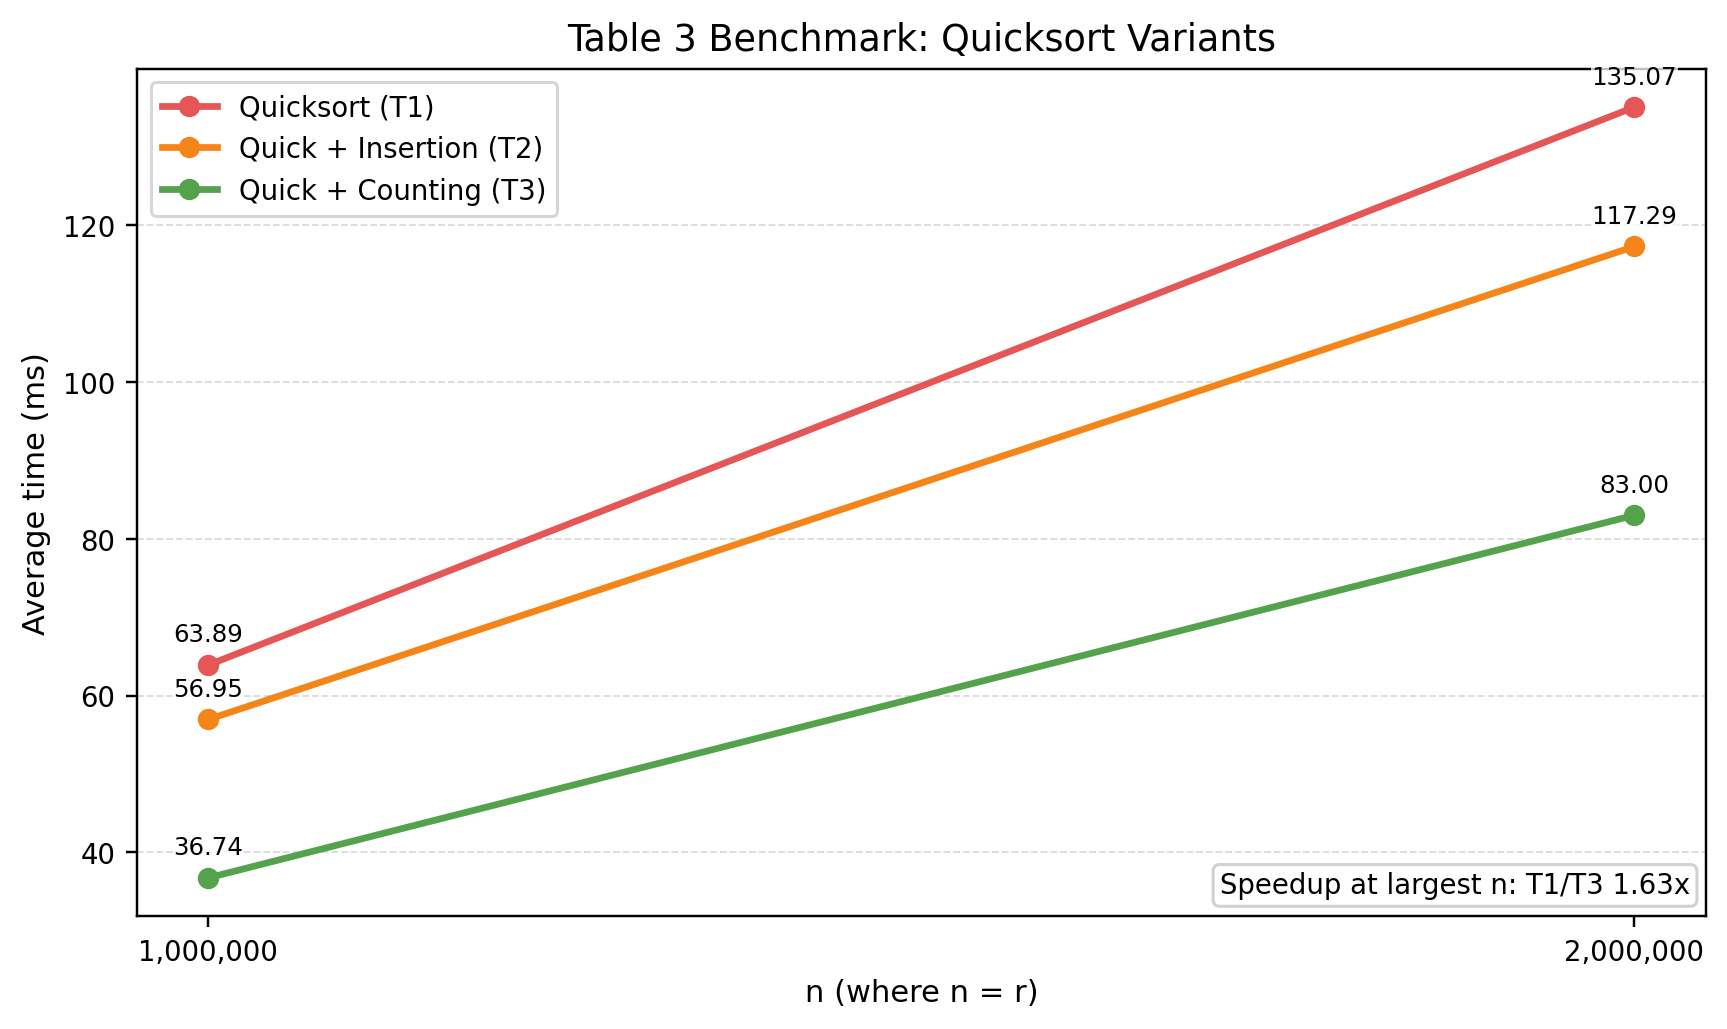
\includegraphics[width=0.78\textwidth]{graphs/table3_quicksort_variants_ms.png}
        \caption{Table 3 trend: quicksort + counting sort is the fastest option at the tested
        sizes.}
        \label{fig:table3trend}
    \end{figure}

    Overall, the results match the main idea of Paper 2. Data locality clearly matters,
    quick+counting works well when $n=r$ is large, and the Table 2.1/2.2 comparison shows that
    more cache pressure can change which method is faster.

    \section{Discussion}

    \subsection{How Close We Got}

    \textbf{Table 1.} We matched this result clearly. The gap between random and sorted input is
    obvious and gets larger as the input size grows.

    \begin{table}[H]
        \centering
        \caption{Table 1 replication points aligned with Paper 2-provided sizes (times in ms).}
        \label{tab:table1-paper-points}
        \small
        \begin{tabular}{rrrr}
            \toprule
            $n$ & $r$ & T1 & T2 \\
            \midrule
            1{,}000{,}000 & 1{,}000{,}000 & 8.05 & 6.44 \\
            2{,}000{,}000 & 2{,}000{,}000 & 25.44 & 12.90 \\
            3{,}000{,}000 & 3{,}000{,}000 & 37.24 & 19.96 \\
            \bottomrule
        \end{tabular}
        \normalsize
    \end{table}

    \textbf{Table 2.1.} We only matched this result partly. The hybrid wins at small $n$, but
    classic counting sort becomes faster after that. On our machine, the preprocessing cost seems
    to matter more.

    \begin{table}[H]
        \centering
        \caption{Table 2.1 replication points for Paper 2-style rows ($T1$ = improved total, $T2$ = classic; times in ms).}
        \label{tab:table22-paper-points}
        \small
        \begin{tabular}{rrrr}
            \toprule
            $n$ & $r$ & T1 & T2 \\
            \midrule
            1{,}000 & 1{,}000{,}000 & 1.377 & 1.717 \\
            2{,}000 & 1{,}000{,}000 & 1.026 & 1.101 \\
            3{,}000 & 1{,}000{,}000 & 1.077 & 0.754 \\
            \bottomrule
        \end{tabular}
        \normalsize
    \end{table}

    \textbf{Table 2.2.} With $r=100{,}000{,}000$, the hybrid is faster for all tested values of
    $n$ because classic counting sort has to work with a much larger count array.
    \begin{table}[H]
        \centering
        \caption{Table 2.2 replication points for Paper 2-style rows ($T1$ = improved total, $T2$ = classic; times in ms).}
        \label{tab:table21-paper-points}
        \small
        \begin{tabular}{rrrr}
            \toprule
            $n$ & $r$ & T1 & T2 \\
            \midrule
            1{,}000 & 100{,}000{,}000 & 1.300 & 86.075 \\
            2{,}000 & 100{,}000{,}000 & 0.828 & 80.146 \\
            3{,}000 & 100{,}000{,}000 & 1.454 & 80.376 \\
            \bottomrule
        \end{tabular}
        \normalsize
    \end{table}

    \textbf{Table 3.} We matched this result clearly as well. Quick+counting is faster than both
    quicksort baselines.

    \begin{table}[H]
        \centering
        \caption{Table 3 replication points for Paper 2-style rows (times in ms).}
        \label{tab:table3-paper-points}
        \small
        \begin{tabular}{rrrr}
            \toprule
            $n=r$ & T1 & T2 & T3 \\
            \midrule
            1{,}000{,}000 & 63.718 & 57.562 & 26.964 \\
            2{,}000{,}000 & 132.881 & 117.656 & 59.648 \\
            \bottomrule
        \end{tabular}
        \normalsize
    \end{table}

    \subsection{Why Our Numbers Differ}

    Our timings do not exactly match the paper because the hardware, cache sizes, JVM behavior,
    and benchmark settings are different. These differences move the crossover points, especially
    between Table 2.1 and Table 2.2, but they do not change the main trend.

    \subsection{What We Learned}

    The hybrid works well in the right setting, but it is not always better than classic counting
    sort. It helps most when cache pressure is high. The threshold $C$ should be tuned for the
    machine and the workload.

    \section{Conclusion}

    We implemented Paper 2's hybrid method and reproduced its main trends on our machine. The main
    lesson is simple: memory behavior matters. For large $n=r$, quick+counting worked best. For
    the $r \gg n$ case, the better method depended on how much pressure the count array put on the
    cache. A sensible next step would be to tune $C$ more carefully and report confidence
    intervals as well as averages.

\end{document}
